\documentclass{article}
\setlength{\parskip}{5pt} % esp. entre párrafos
\setlength{\parindent}{0pt} % esp. al inicio de un párrafo
\usepackage{amsmath} % mates
\usepackage{url} % que las URLs se vean lindos
\usepackage[top=25mm,left=20mm,right=20mm,bottom=25mm]{geometry} % márgenes
\usepackage{parskip}
\usepackage[utf8]{inputenc}
\usepackage[margin=1in]{geometry}
\usepackage{amsmath,amsfonts,amssymb,mathtools}
\usepackage{graphicx,float}
\usepackage{algorithmic}
\usepackage{minted}
\usepackage{subcaption}
\usepackage{multicol}
\usepackage{listings}
\usepackage{xcolor}
\usepackage[sort&compress,numbers]{natbib} % referencias
\usepackage{minted}
\usepackage{hyperref} % ligas de URLs
\usepackage{graphicx} % poner figuras
\usepackage[spanish]{babel} % otros idiomas
\usepackage{listings}
\author{Raul L.} % author
\title{Pr\'{a}ctica 8: modelo de urnas} %título
\date{\today}
\begin{document} % inicia contenido

\maketitle % cabecera


\section{Introducci\'{o}n}\label{intro} % sección y etiqueta
La octava práctica es sobre fenómenos de coalescencia y fragmentación, donde partículas se unen para formar cúmulos y estos cúmulos se pueden volver a descomponer en fragmentos menores. Esto es relevante en muchos campos de química, como por ejemplo en el filtrado de aguas residuales, donde solamente los cúmulos de suficiente tamaño serán capturados por el filtro y hay que buscar formas para facilitar que crezcan los cúmulos de residuos para lograr su filtrado adecuado.

Vamos a suponer que tenemos una cantidad total de 
$n$ partículas y que al inicio el tamaño de los $k$ cúmulos existentes sigue la distribución normal. Para lograr esto, vamos a crear $k$ valores de la distribución normal estándar (media cero, desviación estándar uno) y luego normalizarlos para convertirlos en enteros positivos que sumen a $n$\citep{2}.
\newline

\section{Objetivo}
Supongamos que cúmulos con $c$ o más partículas (haciendo referencia al tamaño crítico $c$ ) son suficientemente grandes para filtrar. Estudia el efecto de la tasa $n$/$k$, usando por lo menos cinco valores distintos para ella, el porcentaje de las partículas que se lograría filtrar por iteración.\citep{2}.

\section{C\'{o}digo}
Para este código se utilizó como base el código de la doctora donde se hicieron modificaciones variando el porcentaje de $k$ y $n$.

 Código en Python 

\url{https://github.com/satuelisa/Simulation/blob/master/UrnModel/aggrFrag.py}

{\bf Código creado en Python}

\url{https://github.com/Raullr28/Resultados/blob/main/P8/practica_8.py}

\renewcommand{\listingscaption}{Código}

\begin{listing}[H]
\begin{minted}{python}

densidad=[(100,1000000),(300,5000),
          (55000,1500000),(7000,35000),(30000,10000000)]
replicas=150
data=[]
for k,n in densidad:
    print("########### k,n:",k,n,"#################")
    prom_rep=[]
    antes= time()
    for rep in range(replicas):
        orig = np.random.normal(size = k)
        cumulos = orig - min(orig)
        cumulos += 1 # ahora el menor vale uno
        cumulos = cumulos / sum(cumulos) # ahora suman a uno
        cumulos *= n # ahora suman a n, pero son valores decimales
        cumulos = np.round(cumulos).astype(int) # ahora son enteros
        diferencia = n - sum(cumulos) # por cuanto le hemos fallado
        cambio = 1 if diferencia > 0 else -1

  \end{minted}
  \label{lst:fibo}
  \caption{Representación de la función y parámetros utilizados.}
  
  
\end{listing}
\renewcommand{\listingscaption}{Código}
\begin{listing}[H]

\begin{minted}{python}
 
 duracion = 50
        digitos = floor(log(duracion, 10)) + 1
        porcen=[]
        for paso in range(duracion):
            assert sum(cumulos) == n
            assert all([c > 0 for c in cumulos]) 
            (tams, freqs) = np.unique(cumulos, return_counts = True)
            cumulos = []
            assert len(tams) == len(freqs)
            for i in range(len(tams)):
                cumulos += romperse(tams[i], freqs[i]) 
 
  \end{minted}
  \label{lst:fibo}
  \caption{Representación ciclo de la partícula.}
\end{listing}
\newpage
% Computational Results
\section{Resultados}
En una gráfica de violines se graficó los resultados del comportamiento de las diferentes $k$/$n$ respectivamente para poder ver su comportamiento con un número alto de repeticiones para poder lograr ver mejores los violines.
%%%%%%%%%%%%%%%%%%%%% imagen 1
\begin{figure}[H]
\centering
\begin{subfigure}[b]{1.0\linewidth}
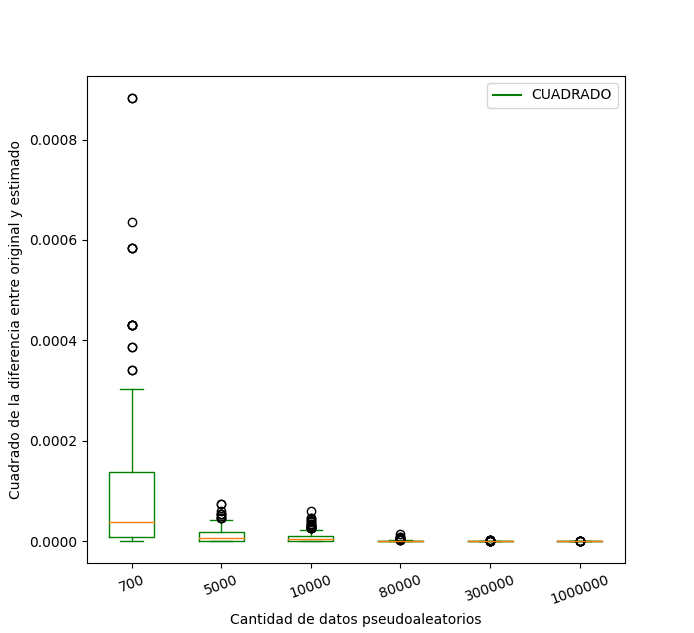
\includegraphics[width=\linewidth]{Imagenes/Figure_2.png}
\end{subfigure}
\caption{función 3D.}
\label{fig:westminster}
\end{figure}
%%%%%%%%%%%%%%%%%%%%%%%  final 


\newpage
\section{Reto 1}
 Un primer reto, determina cómo el momento idóneo de filtrado depende del valor de $c$. ¿Qué todo cambia y cómo si $c$ ya no se asigna como la mediana inicial sino a un valor menor o mayor?.


\section{Resultados}
Paro poder llevar a cabo el reto numero uno se varió el dato c, en dos nuevos valores.
 %%%%%%%%%%%%%%%%%%%%% imagen 6
\begin{figure}[H]
\centering
\begin{subfigure}[b]{1.0\linewidth}
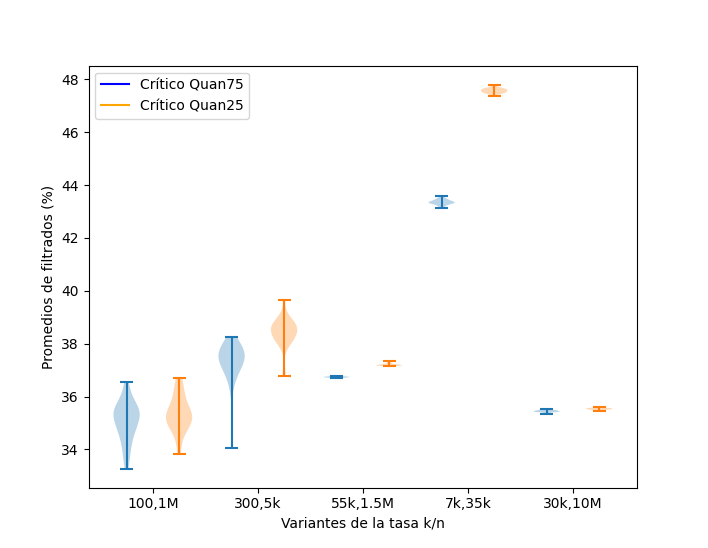
\includegraphics[width=\linewidth]{Imagenes/Figure_r1.png}
\end{subfigure}
\caption{función 3D.}
\label{fig:westminster}
\end{figure}
%%%%%%%%%%%%%%%%%%%%%%%  final

\newpage
\section{Reto 2}

Como el segundo reto, estudia el efecto del parámetro suavizante $d$ en el desempeño de filtrado si la meta es recuperar la mayor cantidad posible de partículas en el proceso. ¿En cuál iteración es conveniente realizar el filtrado? Incluye visualizaciones para justificar las conclusiones.
 
\section{Resultados}
demostrando tamaños de filtros encontrando el mejor tamaño para filtrar la mejor cantidad de cumulos.
 %%%%%%%%%%%%%%%%%%%%% imagen 6
\begin{figure}[H]
\centering
\begin{subfigure}[b]{1.0\linewidth}
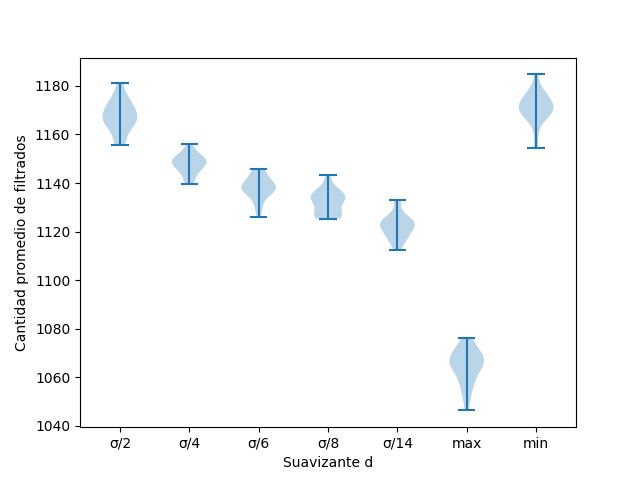
\includegraphics[width=\linewidth]{Imagenes/Figurer2.png}
\end{subfigure}
\caption{función 3D.}
\label{fig:westminster}
\end{figure}
%%%%%%%%%%%%%%%%%%%%%%%  final



\newpage
 \section{Conclusión}
Se mostró con gráficas de violín el comportamiento de diferentes $k$/$n$, se cambió el valor de nuestra $c$ para poder determinar mejores valores y en nuestro ultimo reto se determinó el mejor valor para nuestro filtro.. 
.

 \bibliography{biblio.bib}
 \bibliographystyle{unsrtnat}

 \end{document}


